\documentclass[14pt]{report}
\usepackage{geometry}                % See geometry.pdf to learn the layout options. There are lots.
\geometry{letterpaper}                   % ... or a4paper or a5paper or ... 
%\geometry{landscape}                % Activate for for rotated page geometry
%\usepackage[parfill]{parskip}    % Activate to begin paragraphs with an empty line rather than an indent
\usepackage{graphicx}
\usepackage{amssymb}
\usepackage{epstopdf}
\DeclareGraphicsRule{.tif}{png}{.png}{`convert #1 `dirname #1`/`basename #1 .tif`.png}

\title{MLPR Assignment}
\author{I.D s0840844}
%\date{}                                           % Activate to display a given date or no date
\DeclareMathSizes{10}{10}{9}{8}
\begin{document}
\begin{flushleft}

%\section{}
%\subsection{}
\section { Bayesian Analysis of Uniform distribution}

Given  
$ p(\theta) \sim Pa(b,K) $= \left\{ \begin{array}{rcl} \frac{Kb^k}{\theta^{K+1}}   & \mbox{for } \theta \geq b  \\ 0 & \mbox{otherwise} \end{array}\right


Now with the above Pareto prior, the joint distribution of $\theta$ and $D =\{ x_1,x_2,....x_N\}$ is:
\[ p(D,\theta) =P(D|\theta)P(\theta) = \left\{ \begin{array}{rcl} \frac{1}{\theta^N} . \frac{Kb^K}{\theta^{K+1}} &\mbox { for }  \theta \geq max(max(D),b) \\0 & \mbox{otherwise} \end{array}\right

With the given definition of $P(D)$ and taking $m=max(D)$ , the posterior  $p(\theta|D)$ can now be defined as follows:
\begin{flushright}
\begin{eqnarray*}
 p(\theta|D) = \frac{P(\theta,D)}{P(D)}&=&  \left\{  \begin{array}{rcl}\frac{\frac{1}{\theta^N} . \frac{Kb^K}{\theta^{K+1}}}{\frac{K}{(N+K)b^N}} & \mbox{for  } b\geq m \mbox{ and } b\leq \theta \\ \frac{\frac{1}{\theta^N} . \frac{Kb^K}{\theta^{K+1}}}{\frac{Kb^K}{(N+K)m^{N+K}}} & \mbox{for  } m > b \mbox{ and } m\leq \theta \end{array}\right \\ 0 \mbox{ otherwise}\\
 \end{eqnarray}
 \end{flushright}
 This can be simplified and written as: 
 \begin{flushright}
 \begin{eqnarray*}
 p(\theta|D) = \frac{P(\theta,D)}{P(D)}&=& \left\{ \begin {array}{rcl} \frac{(N+K)b^{N+K}}{\theta^{N+K+1}} \mbox{ for }  b\geq m \mbox{ and } b\leq \theta\\
  \frac{(N+K)m^{N+K}}{\theta^{N+K+1}} \mbox{ for }  m > b \mbox{ and } m\leq \theta \\    \end{array}\right
\end{flushright}  
 
\end{eqnarray}
Note : For b $\geq$ m , $p(\theta|D)$ =0 for $\theta < b$ and similarly for $ m > b$ $   p(\theta|D) =0 $ for $\theta < m$.

The posterior in fact has the same function functional form as a Pareto distribution :
 
 We know the Pareto distribution, Pa is defined as : $ Pa(\alpha, n) =  \frac{\alpha n^\alpha}{\theta^{\alpha+1}}$. If we compare this with the above distribution, we can see $\alpha \equiv  (N+K)$ and $n \equiv \{ m,b\}$

\section{The Tramcar problem}
\subsection{Part A}

Assumptions made: 
\begin{itemize}
\item trams are numbered sequentially as integers starting from 0 to some upper bound $\theta$. Thus the likelihood function $p(x)$ can be defined as:

\[ p(x) = f (x|\theta) = \left\{ \begin{array}{rcl} \frac{1}{\theta} \mbox { for } 0 \leq x \leq \theta \\ 0  \mbox{ otherwise} \end{array}\right\]

\item K=1 and b=1 and the D=\{100\} .
This implies m= 100 
\end{itemize}
Since $ m>b$ the posterior $p(\theta|D)$ is given as :
\[ p(\theta|D) =   \frac{(N+K)m^{N+K}}{\theta^{N+K+1}} = \frac{2. 100^2}{\theta^3} \]

\subsection{Part B}
The posterior $p(\theta|D)$ as shown above is a Pareto distribution. Hence the mean and maximum posterior of   $p(\theta|D)$ can derived using the properties of a Pareto distribution.

\[ \mu (mean) =\frac{(N+K)m}{N+K-1} = \frac{2m}{1} = 200\]
\[ MAP = mode = m = 100\]

\subsection{Part C}
The predictive  density  is given by $p(x|D) = \int_{0}^{\infty} p(x|\theta)p(\theta|D)d\theta$.

As already stated in part A , $p(\theta|D)=0$ for $\theta <m$ thus 
\begin {eqnarray*}
 p(x|D) & =& \int_{m}^{\infty} p(x|\theta)p(\theta|D)d\theta\\
 p(x|D) &	       =&   \int_{100}^{\infty} \frac {1}{\theta} . \frac{2. 100^2}{\theta^3} d\theta \\
                     &=& [ \frac{-2.100^2}{3.\theta^3}]_{100}^{\infty}\\
                     &=& \frac {2}{3.100} \\
                     &=& \frac{1}{150}
\end{eqnarray}

\subsection{Part D}
 From Part C, it is clear that the predictive distribution $p(x|D)$ is a uniform distribution $U(x,\theta)$  where $\theta= 150$:
  
\[ p(x|D)  = \left\{ \begin{array}{rcl} \frac{1}{150} \mbox { for } 0 \leq x \leq 150 \\
 0   \mbox{ otherwise } &\\
  \end{array}\right\]

Therefore for a new data point \textbf{x}, the prediction is :
\[ p(\textbf{x} | D) = \frac{1}{150} \large{I}(\textbf{x} \in [0,150]) =  \frac{1}{150} \large{I}(\textbf{x} \leq150)\]

For observations whose value lie outside 150, the probability of observing them given the dataset D is 0.
Thus $p(50|D)$ =$\frac{1}{150}$ and $p(500|D)$ =0.

\subsection{Part E}
As K \longrightarrow 0 

$\lim_{ K \rightarrow 0}p(\theta)  =0$. Thus the limit of  posterior $p(\theta|D) $ when K tends to 0  :

\[ \lim_{ K \rightarrow 0} p(\theta|D)= \frac{P(\theta,D)}{P(D)}&=& \left\{ \begin {array}{rcl} \frac{(N)b^{N}}{\theta^{N+1}} \mbox{ for }  b\geq m \mbox{ and } b\leq \theta\\
  \frac{(N)m^{N}}{\theta^{N+1}} \mbox{ for }  m > b \mbox{ and } m\leq \theta \\    \end{array}\right

Observations:
\begin{itemize}
\item As $K \rightarrow 0$,  the posterior $p(\theta|D)$ at the limiting value of K is still a Pareto distribution.  Sending K to 0 tends to change only the shape parameter of the original posterior distribution which is illustrated as follows:

We know $ Pa(\kappa, n) =  \frac{\kappa n^\alpha}{\theta^{\kappa+1}}$.

By comparing the above distribution with our original posterior $p(\theta|D)$, we concluded that $ \kappa \equiv (N+K) $ but as K\rightarrow 0    $ \kappa \equiv N$  



By observing the graph below ( where x denote $\theta$), we can see that decreasing the value of the shape parameter $\kappa$ makes the distribution more heavily tailed.  Thus, rare instances will have a greater probability mass assigned to them than before.  Having the posterior  $p(\theta|D)$  more heavily tailed  improves the predictive density that we computed in Part C.


\[\lim_{k\rightarrow 0} p(x|D) =   \int_{100}^{\infty} \frac {1}{\theta} . \frac{1. 100^1}{\theta^2} d\theta = \frac{1}{200}\]
Therefore for a new data point \textbf{x}, the prediction is :
\[ p(\textbf{x} | D) = \frac{1}{200} \large{I}(\textbf{x} \in [0,200]) =  \frac{1}{200} \large{I}(\textbf{x} \leq200)\]
Although the individual probability of observing each individual tram within the range [0-150] is less than before, by assigning probability masses on trams between 150 and 200, the predictor improves prediction by increasing the set of trams that it believes that we might see next. In other words the predictor moves towards the true uniform distribution.


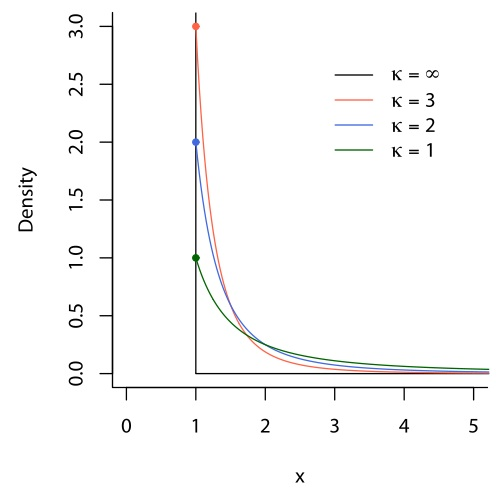
\includegraphics[ scale=0.5]{Pareto.jpg}



\end{itemize}
\section{Bayesian Classification}
Given :

Initially expert1's knowledge regarding the probability of a food delivery being Soylent Red rather than Soylent Yellow is given by a beta distribution with parameters $(n_0,n_1) =(10,10)$ while expert2's initial knowledge is best described by the beta distribution with parameters  $(n_0,n_1) =(100,20)$. 

Hence expert 1's prior belief is captured by $p(f) =f^{(10)-1}(1-f)^{(10)-1}$ where $f $ is probability of seeing Soylent Red.
and  expert 2's corresponding prior belief  is given by $p(f) =f^{(100)-1}(1-f)^{(20)-1}$.


The prior distributions of both experts is shown in figure1.

\begin{figure}[h!]
  \caption{Prior beliefs of Expert1 and Expert2.}
  \centering
    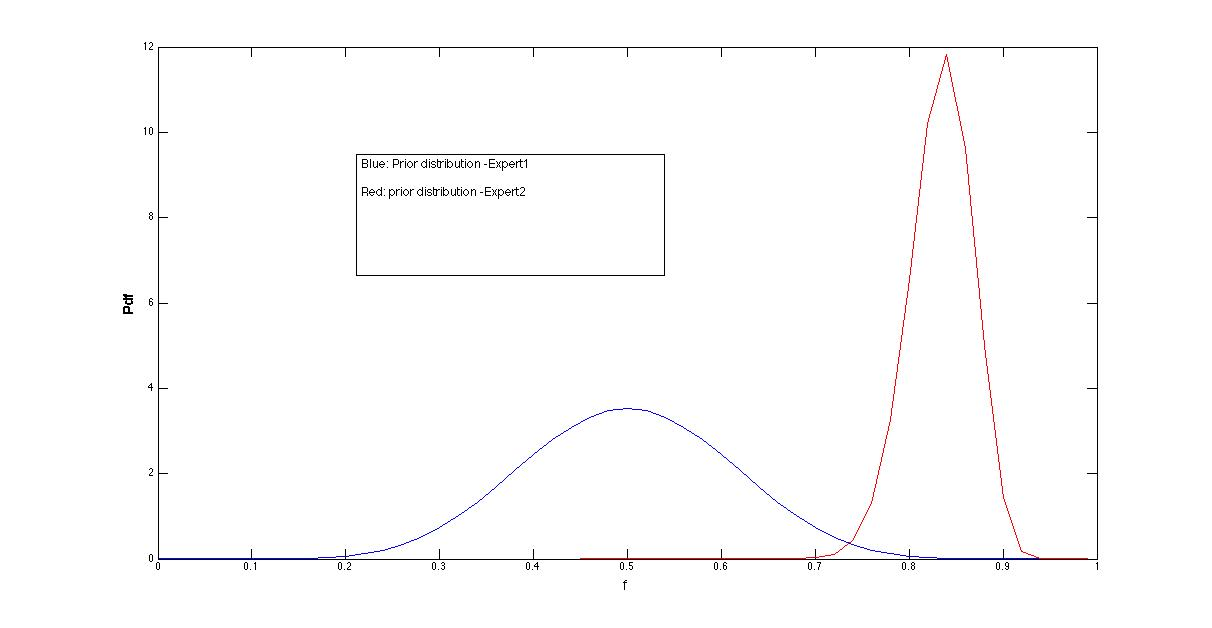
\includegraphics[width=0.8\textwidth]{3p.jpg}
\end{figure}
Observation
\begin{itemize}
\item  Since the true value of $f$ is $\frac{3}{4}$, it can be seen that expert 2 initially has a better opinion.

Reason:
Without seeing any data, if both experts were asked to predict the probability Soylent Red, then on average both experts will chose a value of $f$ that is equal to the mean of the prior distribution. The mean of expert 1's prior distribution is $\frac{1}{2}$ whereas for expert2  the mean of the beta distribution  is $\frac{100}{120}$. The expected value of the prior distribution for expert2 is closer to the true value. Hence, judging from these values taken by the means it can be observed that expert 1 believes that on average  he will see equal number of Soylent Reds and Soylent yellows whereas Expert2  believes on average he will see more Soylent reds than Soylent yellows.
\end{itemize}
\subsection{Computing the posterior}
With incoming data, the posterior distribution of both experts is given by:
\begin{eqnarray*}
 p(f|\textbf{X}) &\varpropto& p(\textbf{X}|f)p(f)\\
 	& =                  & f^k(1-f)^{N-k} f^{n_0 -1}(1-f)^{n_1 -1} \\
	& =                   &  f^{(k+n_0)-1}(1-f)^{(N+n_1-k)-1}
 \end {eqnarray} 
here k represents the number of food items seen  that correspond to Soylent red and N corresponds to the total number of observations that has been made so far..

For Expert 1, the corresponding posterior distribution is given by: $p(f|X) =f^{(k+10)-1}(1-f)^{(N+10-k)-1}$ 

And similarly, for expert 2 the corresponding posterior distribution is  : $ p(f|X)= f^{(k+100)-1}(1-f)^{(N+20-k)-1}$

Note: 
The mean and mode of the posterior distributions of both experts change as more  observations made. The mean of the posterior  distribution for expert 1 is $\mu_1 =\frac{K+10}{N+20} $ and similarly the mean of the posterior distribution of expert 2 is $\mu_1 =\frac{K+100}{N+120}$. The terms $K$ and $N$ change with more data arrives. Hence, we can conclude that the expectation of seeing a Soylent red rather than Soylent yellow change as they continue seeing new data. This is illustrated by the graph in figure 2.

Observation:
The mean of the posterior distribution $p(f|X)$ for both experts  converge  toward the true value of $f$ as the number of observations increase. This is because the two parameters $k$ and $N$ tends to dominate the numerator and denominator in the expression used to compute the mean  $ \mu  =\frac{k+n_0}{N+n_1}$ as the number of samples increase.


\begin{figure}[h!]
  \caption{Empirical posterior mean $\mu$  over  k against N }
  \centering
    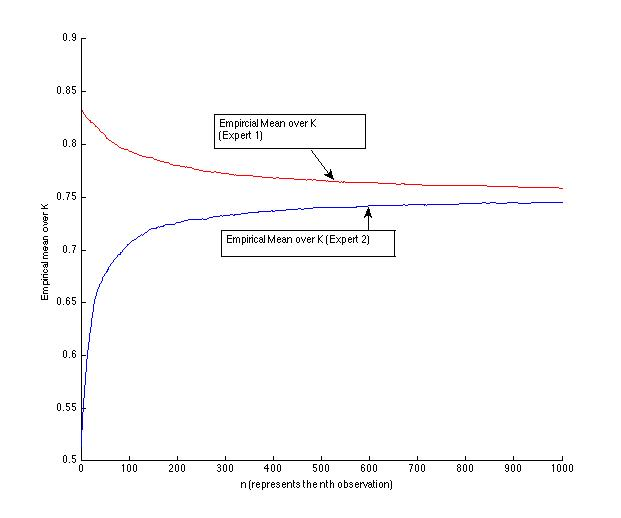
\includegraphics[width=0.8\textwidth]{3A.jpg}
\end{figure}

\subsection{Nature of Convergence}

Observation:
On careful observation of the plots given by figure 3( where the  posterior mean of each expert at the kth simulation, computed after the nth observation, is presented by the y axis), it can be deduced that the posterior distribution of expert 1 is more responsive to incoming data than that of expert 2's posterior distribution.

Reason : The mean and mode of a beta distribution is given by:
\[mu  =\frac{k+n_0}{N+n_1} \mbox{ and }  mode  =\frac{k+n_0-1}{N+n_1-2} \]
The parameter  $n_0 >> n_1$ in expert 2's posterior distribution and this in fact has a substantial impact on the beliefs of the second expert. Since $n_0 >> n_1$,  a  large of number of observations have to be made  to see substantial changes in the value of the mode and mean of the expert 2's posterior distribution. But this is  not the case for expert 1 where  $n_0 =n_1$,  Hence  the sharp initial slopes of the blue plots after the initial observations clearly show that expert 1's posterior distribution is more sensitive to the data. Further evidence to support this claim can found by observing that the blue plots saturate towards the true value  earlier than the red plots. 


\begin{figure}[h!]
  \caption{The posterior mean $p_{exp}$ for each k against  N  }
  \centering
    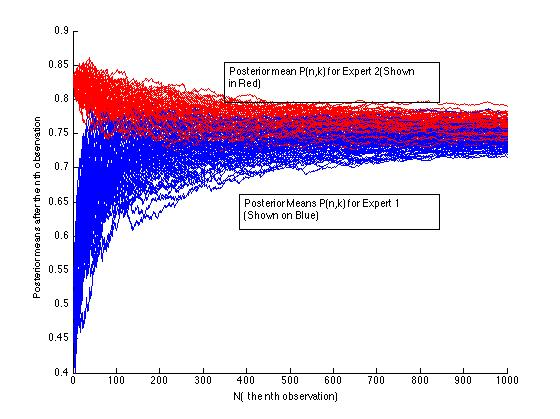
\includegraphics[width=0.8\textwidth]{3B.jpg}
\end{figure}



\subsection{Uncertainty in the long run}
Observation :
From the observation of the plots shown by figure 4 and figure 5, it is clear that the degree of uncertainty regarding the value of $f$ decreases in the long run. This can seen from the decrease in the size of the standard deviation and variation as N increase. The posterior distribution of both experts  thus become narrower  with increasing N and their means  move slowly toward $f=0.75$ with the increasing number of observations. Intuitively, both experts become more and more sure about the true probability distribution as they encounter more data.

\newpage


\begin{figure}[h!]
  \caption{The mean (\underline{+}) standard deviation of the posterior at k=1 against N}
  \centering
    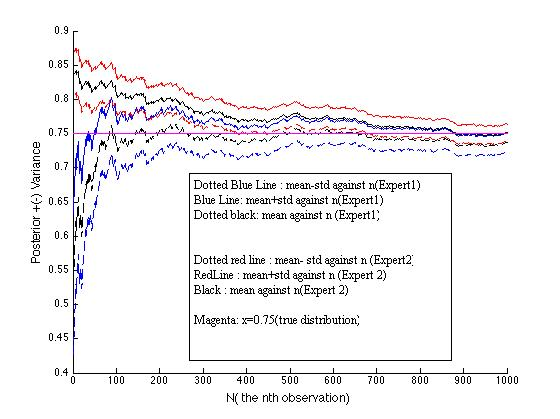
\includegraphics[width=0.8\textwidth]{3C.jpg}
\end{figure} 

\begin{figure}[h!]
  \caption{The variance of the posterior at k=1 against N }
  \centering
    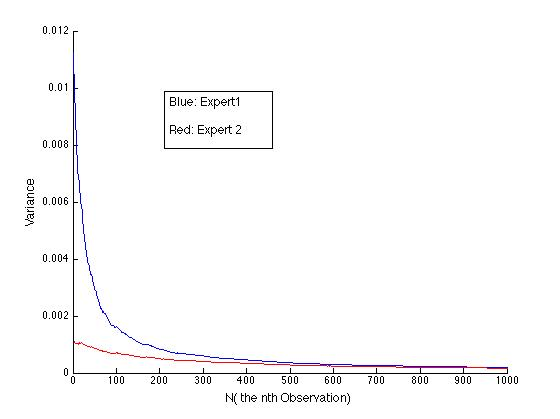
\includegraphics[scale =0.5]{3C2.jpg}
    \end{figure} 




\newpage
\section{Bayesian regression}
The models considered in this last section are  linear regression models. The main property of such models is that the prediction $f(x;w)$ is a linear function of weights 
\[ y(x,w) = \sum_{j=1}^{j=N} w_j\phi_j(x)    + w_0\] where $\phi_j(x)$ are basis functions

The above expression can be written in matrix form by introducing a dummy basis function  $\phi_0(x)=1$ to account the parameter $w_0$ :
\[ f(x,w) = \sum_{j=0}^{j=N} w_j\phi_j(x) =\textbf{w}^{T}\Phi \]
where $\Phi = (\phi_0,\phi_1...\phi_M)$ and $\textbf{w} =(w_0,w_1....w_M)$(M denotes the number of basis functions used)
\subsection{Part A}
\begin{figure}[h!]
  \caption{Functional fits together with the training data against k  }
  \centering
    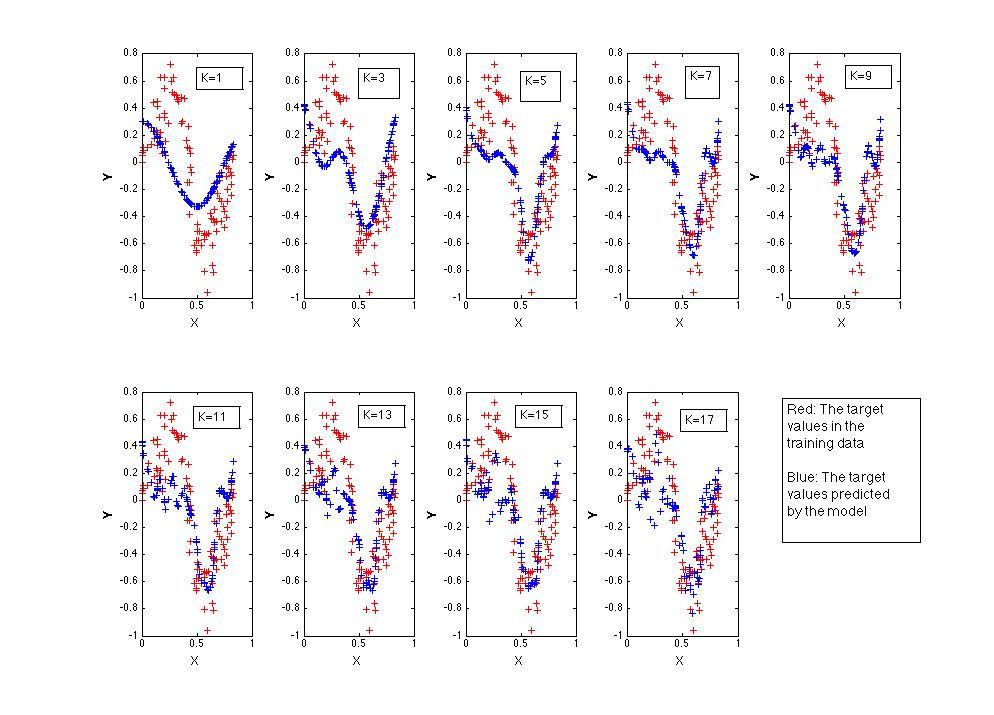
\includegraphics[width=1\textwidth]{4A.jpg}
\end{figure}
The object of Part A is to compare the performance of the prediction $f(x;w)$ on the training data given different linear models. Each model $M_i$ is distinguished from the others only through the number of basis functions it employ i.e M. (All model employ fourier basis functions).
From the observation of figure 6, it can be seen that increasing k i.e M in our case results in the use of linear models that employ more basis functions to ensure that the resulting model gives better fit to the data.  Initially, this proves to be a good heuristic step since since increasing the model complexity not only gives better fits to the training data but also results in better representations of the true function. However, the training data only represents a more portion of the true data space, hence increasing M will inevitably lead to models that overfits the training data. This normally results due to the fact as M increases the magnitude of the coefficients typically gets larger and hence such  flexible models with become increasingly tuned to the random noise on the target values.
\begin{figure}[h!]
  \caption{The Mean squared error against maximum frequency }
  \centering
    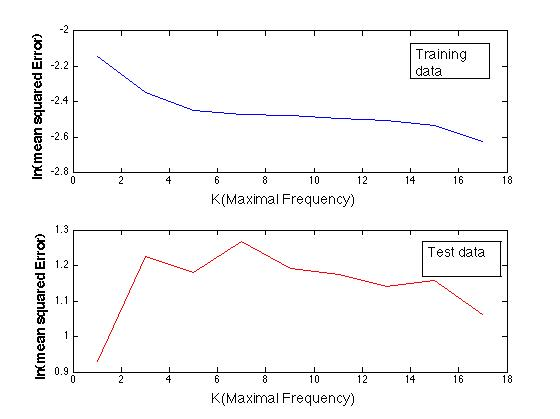
\includegraphics[width=1\textwidth]{4b.jpg}
\end{figure}
\newpage
\subsection{Part B}
\newpage
\subsection {Part C}
As we have seen in Part A and B, using maximum likelihood leads to the choice of parameters $\textbf{w}$ that overfits the data. Through the introduction of the Gaussian prior on the weight, we incorporate a regularisation term that controls the degree of over fitting. The motivation behind this is as follows:

We make an assumption that the target variable y can be explained by the linear model $f(x.w)$ with additive gaussian noise so $ t = f(x;w) + \epsilon$
Hence  consider a data set of inputs $X = {x_1 , . . . , x_N }$ with corresponding target values $y1 , . . . , y_N $ and making the assumption that the points have been drawn independent , the evidence $P(D|M_i)$ is given by
\[ p(D|M_i) = \int p(D,w,M_i)dw  = \int P(D|w,\beta)p(w|\lambda,M_i)dw\]
By keeping the hyper parameters fixed we compute an approximation  of $p(D|M_i)$ by using  $\textbf{w} $ for which $P(D|w,\beta)p(w|\lambda,M_i)$ is max.
The log-likelihood of this approximate $P(D|M_i)$ is:
\[ lnP(D|M_i) = constant  - E(w)\]
where $ E(w) = \frac{\beta}{2} \|\textbf{y} -\Phi\textbf{w}\|^2 + \frac{\lambda}{2}\textbf{w}^T\textbf{w}$
Maximising the log-likelihood is hence equivalent to minimising E(\textbf{w}).

Note : $\lambda$  controls the relative importance of the data dependent error and the regularisation term. Increasing the value of this parameter encourages weight values to decay to 0 thus decreasing the complexity of the model. This counteracts with the large values that set for \textbf{w} when we increase the number of basis functions. From the observation of figure 8, it can be seen that as $\lambda $ increases, the complexity of the model decreases. Hence, the predictive function slowly starts tending towards being linear with increasing $\lamda$.

\begin{figure}[h!]
  \caption{Functional fits using Gaussian prior together with training data against k}
  \raggedleft
    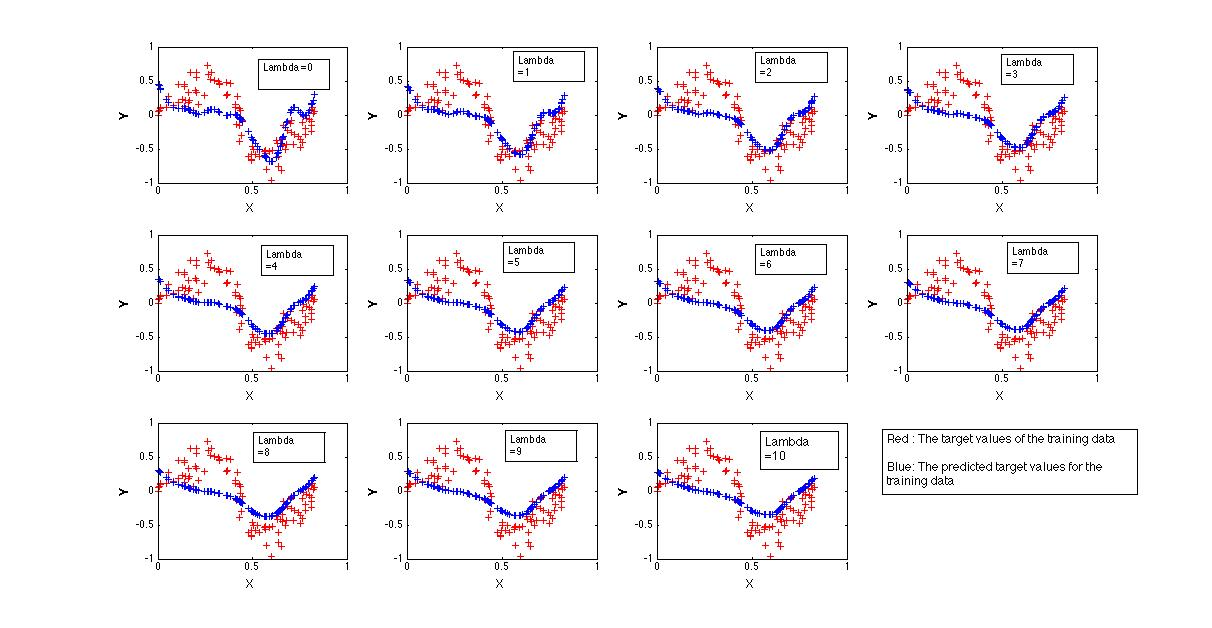
\includegraphics[scale=0.45]{4C.jpg}
\end{figure}





\end{flushleft}

\end{document}  